\section{Fundamentals of Quantum Computation}%
\label{quantum-computation}

Gate-based quantum computation provides means by which to represent exponentially scaling fermionic wavefunctions using polynomially scaling quantum resources. The fundamental idea that permits this is the ability of quantum computers to encode and manipulate superpositions of states. In this section, we will give an introduction to qubits, multiple-qubit states and the elementary quantum gates.

\subsection{Introduction to Qubits}

Classical computation encodes information using binary strings formed from the computational basis states 0 and 1. Thus, given $n$ classical bits, we can encode $2^n$ binary strings. In contrast, information on a quantum computer is encoded using quantum states corresponding to vectors in a two-dimensional complex Hilert space $\mathbb{C}$. The $Z$ eigenbasis $\ket 0$ and $\ket 1$ are the eigenstates of the Pauli $Z$ matrix, and form the computational basis for quantum computation.

\begin{figure}[H]
    \centering
    \begin{minipage}{.45\textwidth}
        \centering
        \includezxdiagramtext{chapter-1/zero}{0.35}{
        \begin{pmatrix} 1 \\ 0 \end{pmatrix}}
    \end{minipage}%
    \begin{minipage}{0.45\textwidth}
        \centering
        \includezxdiagramtext{chapter-1/one}{0.35}{
        \begin{pmatrix} 0 \\ 1 \end{pmatrix}}
    \end{minipage}
    \caption{$Z$ eigenbasis.}
    \label{z-eigenstates}
\end{figure}

An arbitrary qubit state $\ket\psi$ can be described as a complex linear combination of the computational basis states $\ket\psi = \alpha\ket 0 + \beta\ket 1$ provided that the qubit state is normalised, $|\alpha|^2 + |\beta|^2 = 1$. In other words we require two complex numbers ($\alpha$ and $\beta$), or four real numbers, to describe an arbitrary qubit state. Since only the relative phase between the basis states is directly measureable, there is a redundancy in this description that allows us to represent an arbitrary qubit state using only three real numbers.

By taking advantage of this redundancy, we obtain a three-dimensional representation of an arbitrary qubit state, known as the Bloch sphere. Note that opposite points on the Bloch sphere correspond to mutually orthonal states (see the $Z$ eigenbasis in Figure \ref{z-eigenstates}). We could have equivalently chosen any pair of orthonormal states to form the computational basis. For instance, we define the $X$ eigenstates as follows.

\begin{figure}[H]
    \centering
    \begin{minipage}{.45\textwidth}
        \centering
        \includezxdiagramtext{chapter-1/plus}{0.4}{
        \frac{\ket 0 + \ket 1}{\sqrt 2}}
    \end{minipage}%
    \begin{minipage}{0.45\textwidth}
        \centering
        \includezxdiagramtext{chapter-1/minus}{0.4}{
        \frac{\ket 0 - \ket 1}{\sqrt 2}}
    \end{minipage}
    \caption{$X$ eigenbasis.}
    \label{x-eigenstates}
\end{figure}

In theory, a qubit can exist in an infinite number of states, however, upon measuring the qubit state with respect to a particular basis, the qubit state collapses into one computational basis state or the other. This result is known more formally as the \textit{no-cloning theorem}, which states that we cannot create indentical and independent copies of an arbitrary qubit state, as this would involve first measuring that state.

\subsection{Multiple-Qubit States}

Let us now consider systems consisting of multiple qubits. Similarly to how $n$ classical bits give rise to $2^n$ binary strings, we have that $n$ qubits give rise to $2^n$ basis states. These basis states are formed by taking the Kronecker. For instance, a two-qubit system gives rise to the four following basis states.
\begin{equation*}
    \ket{00} = \ket 0 \otimes \ket 0 \qquad
    \ket{01} = \ket 0 \otimes \ket 1 \qquad
    \ket{10} = \ket 1 \otimes \ket 0 \qquad
    \ket{11} = \ket 1 \otimes \ket 1
\end{equation*}
An arbitrary $n$-qubit \textit{state vector}, describing the state of the entire system, can be formed by taking a complex linear combination of the $2^n$ basis states. Therefore, in order to fully describe an arbitrary $n$-qubit state vector, we need to specify $2^n$ complex coefficients. In the case of a two-qubit system, we have the following.
\begin{gather*}
    \ket\psi =
    \alpha \ket{00} +
    \beta \ket{01} +
    \gamma \ket{10} +
    \delta \ket{11} \\
    \text{where} \,\,\,\, \alpha, \, \beta, \, \gamma, \, \delta \in \mathbb{C}
\end{gather*}

\subsection{Introduction to Quantum Gates}%
\label{quantum-gates}

Quantum gates, by definition, correspond to unitary transformations, $U^{-1} = U^\dagger$ \cite{Nielsen2012}. In other words, any quantum gate corresponds to a square unitary matrix that conserves the complex inner product of the state it acts on. Consequently, quantum gates can be viewed as rotations of the qubit state vector in Hilbert space. Let us introduce the most fundamental gates in quantum computation, known as the Pauli gates. The Pauli gates are described by the Pauli matrices: $2 \times 2$ matrices that rotate an arbitrary qubit state by $\pi$ radians about their respective axes.

\begin{figure}[H]
    \centering
    \begin{equation*}
        I = \begin{pmatrix} 1 & 0 \\ 0 & 1\end{pmatrix} \qquad
        X = \begin{pmatrix} 0 & 1 \\ 1 & 0\end{pmatrix} \qquad
        Y = \begin{pmatrix} 0 & -i \\ i & \,\,\,\,0\end{pmatrix} \qquad
        Z = \begin{pmatrix} 1 & \,\,\,0 \\ 0 & -1\end{pmatrix}
    \end{equation*}
    \caption{The Pauli matrices.}
    \label{pauli-matrices}
\end{figure}

The Pauli $X$ gate is the quantum analogue of the classical NOT gate in that it maps $\ket 0 \leftrightarrow \ket 1$. Importantly, the Pauli $X$ differs from its classical counterpart in that it can act on any arbitrary qubit state.

\begin{figure}[H]
    \centering
    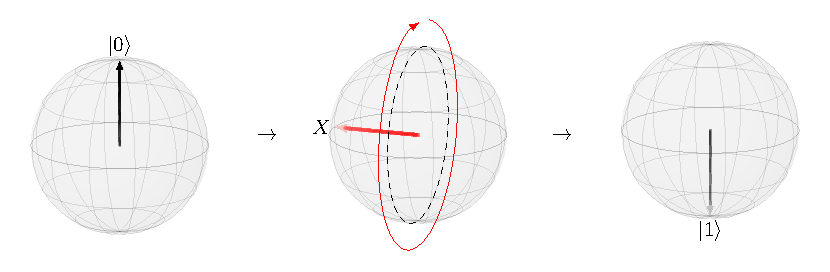
\includegraphics[width=0.6\linewidth]{chapter-1/zero_one}
    \caption{Pauli $X$ gate acting on the $\ket 0$ state.}
\end{figure}

Similarly, we have that the Pauli $Z$ gate maps $\ket + \leftrightarrow \ket -$.

\begin{figure}[H]
    \centering
    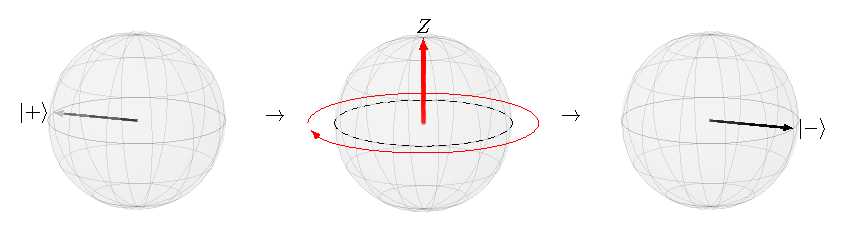
\includegraphics[width=0.6\linewidth]{chapter-1/plus_minus}
    \caption{Pauli $Z$ gate acting on the $\ket +$ state.}
\end{figure}

The Hadamard gate maps $\ket 0 \leftrightarrow \ket +$ and $\ket 1 \leftrightarrow \ket -$. Hence, the Hadamard gate can be viewed as interconverting between the $Z$ and $X$ bases through a rotation $\pi$ radians about the line bisecting the $z$ and $x$ axes in the Bloch sphere representation. Since the Hadamard and Pauli gates correspond to Hermitian matrices, and since all quantum gates are unitary by definition, it follows that they are also self-inverse.

\begin{figure}[H]
    \centering
    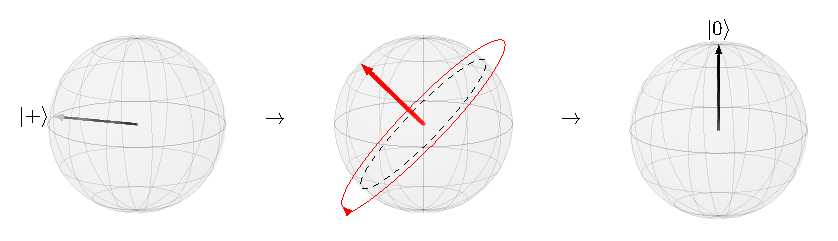
\includegraphics[width=0.6\linewidth]{chapter-1/plus_zero}
    \caption{Hadamard gate acting on the $\ket +$ state.}
\end{figure}

The R$_Z(\theta)$ and R$_X(\theta)$ rotation gates correspond to rotations of the Bloch sphere by some angle $\theta$, in the $Z$ and $X$ bases respectively.

\begin{figure}[H]
    \centering
    \begin{minipage}{0.45\textwidth}
        \centering
        \includezxdiagramtext{chapter-1/z_rotation}{0.4}{
        \begin{pmatrix} 1 & 0 \\ 0 & e^{i\theta} \\ \end{pmatrix}}
    \end{minipage}
    \begin{minipage}{0.45\textwidth}
        \centering
        \includezxdiagramtext{chapter-1/x_rotation}{0.35}{
        \begin{pmatrix}
              1 + e^{i\theta} & 1 - e^{i\theta} \\
              1 - e^{i\theta} & 1 + e^{i\theta}
        \end{pmatrix}}
    \end{minipage}
    \caption{Arbitrary rotations in the $Z$ and $X$ bases by $\theta$ radians.}
\end{figure}

\subsection{Multiple-Qubit Gates}

We will now introduce the two-qubit CNOT gate, which is used to entangle two qubits. Consider a two-qubit state of the form $\ket \alpha \otimes \ket \beta$. We define CNOT as the gate that takes $\alpha$ to be the control qubit and $\beta$ to be the target qubit, and acts on the $\ket\alpha\otimes\ket\beta$ state to give the $\ket\alpha\otimes\ket{\alpha\oplus\beta}$ state. That is, the CNOT gate applies the Pauli $X$ gate to the target qubit \textit{iff} the control qubit is in the $\ket 1$ state. The CNOT gate acts on the two-qubit basis states as follows.
\begin{equation*}
    \ket{00} \rightarrow \ket {00} \qquad
    \ket{01} \rightarrow \ket {01} \qquad
    \ket{10} \rightarrow \ket {11} \qquad
    \ket{11} \rightarrow \ket {10}
\end{equation*}
In this way the CNOT gate is the quantum generalisation of the classical XOR gate. Since the CNOT must be unitary, it has two outputs instead of one, such that $\text{CNOT}^{-1}$ is well-defined.

We define the matrices corresponding to the CNOT gates, with the control and target qubits interchanged, as follows.
\begin{equation*}
\text{CNOT}^{c=0}_{t=1} =
    \begin{pmatrix}
        1 & 0 & 0 & 0 \\
        0 & 1 & 0 & 0 \\
        0 & 0 & 0 & 1 \\
        0 & 0 & 1 & 0
    \end{pmatrix} \qquad
    %
    \text{CNOT}^{c=1}_{t=0} =
    \begin{pmatrix}
        1 & 0 & 0 & 0 \\
        0 & 0 & 0 & 1 \\
        0 & 0 & 1 & 0 \\
        0 & 1 & 0 & 0
    \end{pmatrix}
\end{equation*}\smallskip
The CNOT gate can be used to entangle two qubits when the control qubit exists in a superposition of states. For instance, the CNOT gate actions on the $\ket{+0}$ state to give the $\frac{1}{\sqrt 2} (\ket{00} + \ket{11})$ Bell state.
